\documentclass{article}
\title{Background Literature and Designs}
\author{Michael Buch}
\date{\today}

\usepackage[inline]{enumitem} % inline numbered lists
\usepackage[left=2cm,right=2cm]{geometry}
\usepackage{verbatim} % for comments
\usepackage{graphicx}

\begin{document}
\maketitle
\frenchspacing

\newcommand{\mslang}{$\lambda\uparrow\downarrow$}
\newcommand{\mslangStar}{$\lambda\uparrow\downarrow^*$}

\section{About this document}
This is a collection of references and summaries to research in the field of meta-programming/supercompilation/partial evaluation

\section{Examples}
Examples drawn from paper on collapsing towers \cite{amin2017collapsing}:
\begin{itemize}
	\item Regular expression matcher <- Evaluator <- Virtual Machine
	\begin{itemize}
		\item Generate low-level VM code for a matcher specialized to one regex (through arbitrary number of intermediate interpreters)
	\end{itemize}
	\item Modified evaluator <- Evaluator <- Virtual Machine
	\begin{itemize}
		\item Modified for tracing/counting calls/be in CPS
		\item Under modified semantics "interpreters become program transformers". E.g. CPS interpreter becomes CPS transformer
	\end{itemize}
\end{itemize}

\section{Methodologies}
\begin{itemize}
	\item Stage polymorphism \cite{ofenbeck2017staging}: ``abstract over staging decisions'' i.e. single program generator can produce code that is specialized in many different ways (instance of the Fourth Futamura Projection? \cite{gluck2009there}) 
	\item Multi-level base evaluator written in \mslang: supports staging operators (\textbf{polymorphic Lift})
	\item Modify other interpreters: make them \textbf{stage polymorphic}, i.e. commands either evaluate code (like an interpreter) or generate code (like a translator)
	\item Stage only user-most interpreter: \textit{wire tower} such that the \textbf{staging commands in $L_{n}$ are interpreted directly in terms of staging commands in $L_{0}$} i.e. staging commands pass through all other layers handing down commands to layers below without performing any staging commands
	\item Non-reflective method: meta-circular evaluator \textbf{Pink} => collapse arbitrary levels of ``self-interpretation''
	\item \mslang features:
	\begin{itemize}
		\item \textit{run residual code}
		\item binding-time/stage polymorphism \cite{henglein1994polymorphic}
		\item preserves execution order of future-stage expressions
		\item does not require type system or static analysis
		\begin{itemize}
			\item TDPE \cite{danvy1999type} (great explanation also at \cite{grobauer2001second}): \textbf{polymorphic Lift} operator turns static values into dynamic (future-stage) expressions
		\end{itemize}
	\end{itemize}
\end{itemize}

\subsection{Towers of Interpreters Project Overview}
\subsubsection{Scala}
\begin{itemize}
	\item base.scala: implements definitional interpreter for \mslang
\end{itemize}

\section{Results}
\begin{itemize}
	\item Able to achieve compilation of stack-machine on top the Pink evaluator (including tracing evaluator etc.)
	\item Compilation i.e. collapsing through explicit staging annotations requires intricate knowledge of infrastructure and does not support all data structures e.g. stacks
\end{itemize}

\section{Problems}
A useful analogy is the one presented in \cite{amin2017collapsing}: a Python interpreter running on a JavaScript emulator of a x86 CPU. What we envision (with reference to this hypothetical setting) is handling the two following cases:
\begin{enumerate}
	\item A one-off run of a python script on top of this stack should be collapsed by bypassing the emulator interpretation
	\item A continuously running emulator evaluating a continuously running python interpreter should collapse individual runs of interpretation while respecting the dynamically changing environment
	\begin{itemize}
		\item Here a dynamically changing environment also implies side-effects that are capable of changing the semantics of interpreters within the tower at runtime
		\item In literature, the closest to compiling a dynamically changing tower is \cite{asai1997partial, amin2017collapsing} (for a \textit{reflective} language Black) and GraalVM \cite{wurthinger2013one}
	\end{itemize}
\end{enumerate}
To tackle the first of these problems we construct a similar yet condensed form of the setting as shown in \ref{secd_tower_arch}.

\begin{figure}[t]
	\centering
	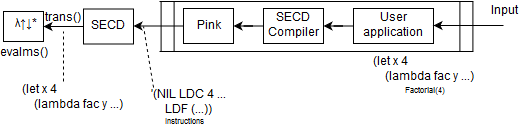
\includegraphics[scale=0.75]{secd_arch.png}
	\caption{``Effectively functional'' \mslangStar with SECD tower above it}\label{secd_tower_arch}
\end{figure}

\section{Contributions}
\begin{itemize}
	\item Extension of the core \mslang to support side effects, combining previous insights into multi-level $\lambda$ \cite{nielson1996multi} and work on side-effects in partial evaluators \cite{asai1997partial}.
	\item Development a CESK-style abstract machine/ abstract interpreter for said extended \mslang
	\item Form a basis for further work on towers by providing a stage polymorphic base evaluator capable of modelling functional or imperative languages
	\item Mimick a practical tower through a SECD machine on top of the base evaluator and show compilation without staging commands throughout the tower
	\item Theoretical proposal of how one might achieve collapsing in practice
\end{itemize}
	
\bibliographystyle{IEEEtran}
\bibliography{lit_review}

\end{document}